% !TeX program = xelatex
\documentclass[11pt,a4paper]{article}
\usepackage{fontspec}
\IfFontExistsTF{Times New Roman}{\setmainfont{Times New Roman}}{}
\IfFontExistsTF{Consolas}{\setmonofont{Consolas}}{}
\usepackage{xeCJK}
\IfFontExistsTF{Harano Aji Mincho}{\setCJKmainfont{Harano Aji Mincho}}{%
  \IfFontExistsTF{Yu Mincho}{%
    \IfFontExistsTF{Yu Mincho Demibold}{%
      \setCJKmainfont[BoldFont={Yu Mincho Demibold},ItalicFont={Yu Mincho},
        BoldItalicFont={Yu Mincho Demibold}]{Yu Mincho}%
    }{\setCJKmainfont[AutoFakeBold=2,ItalicFont={Yu Mincho}]{Yu Mincho}}%
  }{\setCJKmainfont{Noto Serif CJK JP}}}
\IfFontExistsTF{Harano Aji Gothic}{\setCJKsansfont{Harano Aji Gothic}\setCJKmonofont{Harano Aji Gothic}}{%
  \IfFontExistsTF{Yu Gothic}{\setCJKsansfont{Yu Gothic}\setCJKmonofont{Yu Gothic}}{%
    \setCJKsansfont{Noto Sans CJK JP}\setCJKmonofont{Noto Sans CJK JP}}}
\usepackage[top=24mm,bottom=25mm,left=24mm,right=24mm]{geometry}
\usepackage{amsmath,amssymb,booktabs,tabularx,array,graphicx}
\usepackage[font=small,labelfont=bf]{caption}
\usepackage{xcolor}
\usepackage{hyperref}
\definecolor{Accent}{HTML}{1C455B}
\hypersetup{colorlinks=true,linkcolor=Accent,citecolor=Accent,urlcolor=Accent,
  pdftitle={DIY AutoML: 分類モデルの選定・不確かさ・データ品質をつなぐ評価基盤}}
\renewcommand{\figurename}{図}
\renewcommand{\tablename}{表}
\renewcommand{\refname}{参考文献}
\setlength{\parindent}{1em}
\setlength{\parskip}{0.3em}
\clubpenalty=10000
\widowpenalty=10000
\displaywidowpenalty=10000
\linespread{1.16}
\graphicspath{{images/}}
\newcolumntype{Y}{>{\raggedright\arraybackslash}X}
\newcommand{\macroF}{\ensuremath{F_{1,\mathrm{macro}}}}
\newcommand{\project}{DIY AutoML}
\begin{document}
\begin{center}
{\LARGE\bfseries DIY AutoML\par}
\vspace{0.35em}
{\Large\bfseries 分類モデルの選定・不確かさ・データ品質をつなぐ評価基盤\par}
\vspace{0.85em}
{\small 2026年11月19日 \quad 技術論文・初稿\par}
\end{center}

\section*{要旨}
機械学習の性能値を採用判断に使うには、学習と評価に分けた単位、比較対象、誤りの内訳、評価値の不確かさが必要である。\project{}は、データ点検と抽出後の再点検、共通分割での候補比較、保留テスト、固定モデルの区間推定、再検証可能な結果保存を接続する。通信解約データ3,150行では、同一の数値入力をグループ化すると、学習側にも同じ値を持つ保留行が107件から0件になった。自転車貸出データの後続期間582行では、ランダムフォレストと曜日・時間帯の多数決のmacro F1は0.638と0.656だった。「通常」109件の検出数は80件と72件で、月によってmacro F1の大小関係が変わった。補足として、AutoGluonとの照合、TensorFlowとPyTorchの予測確率の比較、焼きなまし法による特徴量探索、16\,GB端末での前処理負荷を報告する。時間依存を考慮した性能差の区間、ラベル確定の遅れ、および独立データでの検証は次の課題である。

\noindent\textbf{キーワード}\quad AutoML、分類評価、グループ分割、日付順評価、ブートストラップ、単純ルール

\section*{Abstract}
DIY AutoML records the path from tabular data inspection and model selection to held-out evaluation and reporting. In an Iranian Churn example with 3,150 rows, grouping identical feature vectors reduced the number of held-out rows with an identical training input from 107 to zero. On a chronological bike-sharing holdout of 582 rows, the selected random forest and a weekday-by-hour majority rule achieved macro F1 scores of 0.638 and 0.656, respectively. The forest detected 80 of 109 regular-demand observations and the rule detected 72. Their relative performance varied by month. Additional experiments examine cross-library agreement, backend probability differences, feature subset search and the cost of data preparation on a 16 GB PC. Temporal uncertainty intervals and external validation remain open.

\section{背景と目的}\label{sec:background}

表形式データの分類には、決定木や線形モデルなど複数の候補を同じ手順で比較する方法がある。AutoGluonのようにモデル選定やアンサンブルを自動化する基盤も使われている\cite{autogluon}。業務で使う際には、性能値の大小に加え、その値がどの対象、どの時点、どの分割で得られたかが判断に影響する。同じ顧客の記録が学習と評価にまたがるときと、新しい顧客を評価するときでは、同じF1でも答える問いが異なる。後続期間に適用する用途では、クラスの割合や入力分布が変わることもある。

本研究の目的は、分類器の選定を自動化し、その選定を支えたデータ点検と分割、単純ルールとの比較、誤分類の内訳をあとから検査できる評価基盤を構築することである。設計上の課題は三つある。第一に、記録の単位や予測時点を確認し、用途に合う分割を選べるようにする。第二に、評価値とその条件付き不確かさを出し、数値計算の差や測定・ラベルの偏りについて、どの範囲まで確認したかを明示する。第三に、単純ルールと同じ保留データで比べ、総合指標の差を見逃しと誤検知に分けて読めるようにする。

11月9日の短報は、モデル選定、固定モデルの条件付きブートストラップ、業務3例を中心に報告した。11月19日の改稿では、データ点検と抽出、グループ分割と日付順評価、Windowsの業務利用者向け画面を加えた\cite{letters,milestone}。本稿は両短報を踏まえ、各評価単位の設計、実験条件、結果の解釈、再実行の入口を一つにまとめる。主要な実証は教師あり分類で行い、バックエンド比較、特徴量探索、負荷測定を補足検証として扱う。

\section{評価基盤の設計}\label{sec:methods}

\subsection{元データの点検と作業用データ}

入力は数値特徴量と分類ラベルを持つCSVである。まずヘッダー、欠損・非有限値、重複、同じ特徴量で正解ラベルが異なる組、クラス別件数を集計する。利用者は1行の意味、何を予測するか、予測時点、管理用IDや観測時刻、ラベルの由来を記録できる。これらは利用者が与える評価条件である。特徴量が実際に予測時点で使えるかは、記録の由来と照合する。

図\ref{fig:workflow}に、点検、評価、利用者別の出力をつなぐ運用を示す。たとえば10万行以上または20列以上を中継ファイルの作成を検討する目安とし、元CSVの読み直しや整形を繰り返す場合に作業用ファイルを再利用する。利用者の希望があれば、規模によらず圧縮ParquetまたはDuckDBファイルへ変換できる。現行版は利用者が変換を指定し、BP向け画面では圧縮Parquetを選べる。学習には選んだ列をCSVに書き出して渡す\cite{audit}。

学習に使う列を選び、行数、欠損、ラベル別件数、同じ入力でラベルが異なる組を再点検する。元CSVを保管し、評価対象の行は原則として全件を使う。欠損のある行を除外する場合は、基準と除外前後の件数を記録する。メモリや時間は学習時の行数、列数、モデルの設定から見積もる。予算を超える場合はモデル候補や計算設定を見直し、収まらなければ実行を保留する。

評価値と実行条件を保存し、同じ結果を用途に応じて提示する。データサイエンティスト（DS）向けにはコンソールの要約と予測・分割などの再分析用データを用意する。ビジネス利用者（BP）向けにはExcelで評価の対象件数、誤りの内訳、比較結果を示し、必要に応じて図を添える。

\begin{figure}[!t]
\centering
\begingroup
\setlength{\unitlength}{1mm}
\setlength{\fboxsep}{0pt}
\setlength{\fboxrule}{0.4pt}
\colorlet{FlowBorder}{Accent!65!white}
\colorlet{FlowStep}{Accent!5!white}
\colorlet{FlowChoice}{orange!12!white}
\colorlet{FlowReview}{black!6!white}
\colorlet{FlowOutput}{Accent!12!white}
% Arguments give the centre, width, height, fill and text, in that order.
\newcommand{\workflownode}[6]{%
  \put(#1,#2){\makebox(0,0){%
    \fcolorbox{FlowBorder}{#5}{%
      \parbox[c][#4mm][c]{#3mm}{\centering\fontsize{8.5pt}{11pt}\selectfont #6}}}}}
\newcommand{\workflowarrowhead}{%
  \begin{picture}(0,0)
    \put(-0.48,0.6){\makebox(0,0){\rotatebox{-51}{\rule{1.55mm}{0.4pt}}}}
    \put(0.48,0.6){\makebox(0,0){\rotatebox{51}{\rule{1.55mm}{0.4pt}}}}
  \end{picture}}
\begin{picture}(160,122)
  \color{FlowBorder}
  \linethickness{0.4pt}
  % Input and the choice of working format.
  \put(116,115){\line(1,0){8}}
  \put(124,115){\rotatebox[origin=c]{90}{\workflowarrowhead}}
  \put(80,110){\line(0,-1){5}}
  \put(80,105){\workflowarrowhead}
  \put(80,93){\line(0,-1){4}}
  \put(28,89){\line(1,0){104}}
  \put(28,89){\line(0,-1){4}}
  \put(80,89){\line(0,-1){4}}
  \put(132,89){\line(0,-1){4}}
  \put(28,85){\workflowarrowhead}
  \put(80,85){\workflowarrowhead}
  \put(132,85){\workflowarrowhead}
  % The three formats converge on the same preparation step.
  \put(28,75){\line(0,-1){4}}
  \put(80,75){\line(0,-1){4}}
  \put(132,75){\line(0,-1){4}}
  \put(28,71){\line(1,0){104}}
  \put(80,71){\line(0,-1){2}}
  \put(80,69){\workflowarrowhead}
  \put(80,59){\line(0,-1){5}}
  \put(80,54){\workflowarrowhead}
  \put(113,49){\line(1,0){5}}
  \put(118,49){\rotatebox[origin=c]{90}{\workflowarrowhead}}
  \put(80,44){\line(0,-1){4}}
  \put(80,40){\workflowarrowhead}
  % Both outputs use the saved evaluation.
  \put(80,28){\line(0,-1){5}}
  \put(40,23){\line(1,0){80}}
  \put(40,23){\line(0,-1){4}}
  \put(120,23){\line(0,-1){4}}
  \put(40,19){\workflowarrowhead}
  \put(120,19){\workflowarrowhead}

  \color{black}
  \workflownode{80}{115}{72}{10}{FlowStep}{\textbf{元CSVを保管して点検}}
  \workflownode{142}{115}{35}{10}{FlowReview}{不備があれば\\点検結果を返す}
  \workflownode{80}{99}{72}{12}{FlowChoice}{\textbf{中継データを作るか}\\規模・再利用・利用者指定}
  \workflownode{28}{80}{45}{10}{FlowStep}{元CSVを使う}
  \workflownode{80}{80}{45}{10}{FlowStep}{圧縮Parquetに変換}
  \workflownode{132}{80}{45}{10}{FlowStep}{DuckDBファイルに変換}
  \workflownode{80}{64}{88}{10}{FlowStep}{学習用の列を選び、欠損と件数を再点検}
  \workflownode{80}{49}{66}{10}{FlowChoice}{\textbf{対象行を保ったまま学習できるか}}
  \workflownode{138}{49}{39}{12}{FlowReview}{設定を見直す\\収まらなければ保留}
  \workflownode{80}{34}{104}{12}{FlowStep}{\textbf{保留データを確保し、学習側の交差検証で順位付け}\\保留評価と不確かさの結果を保存}
  \workflownode{40}{11}{72}{16}{FlowOutput}{\textbf{DS向け}\\コンソール要約・再分析用データ}
  \workflownode{120}{11}{72}{16}{FlowOutput}{\textbf{BP向け}\\Excel要約・必要に応じて図}
\end{picture}
\endgroup
\caption{データ点検からDS・BP向け出力までの運用フロー。中継形式と学習条件は利用者が指定する。}
\label{fig:workflow}
\end{figure}


\begin{table}[htbp]
\centering
\small
\caption{工程と、あとから確認する主な記録}
\label{tab:pipeline}
\begin{tabularx}{\linewidth}{@{}p{31mm}YY@{}}
\toprule
工程 & 確認する内容 & 保存する情報 \\
\midrule
元CSVの点検 & 欠損、重複、ラベル別件数と評価条件 & 入力のハッシュ、点検Excel、JSON \\
抽出と再点検 & 使う特徴量、行数、クラス構成 & 抽出条件、抽出CSV、再点検の結果 \\
モデル選定 & 学習側の共通分割と候補ごとの指標 & 設定、検証行、平均と区間ごとの成績 \\
保留テスト & 選定モデルと単純ルールの結果 & 予測、正解、誤りの件数、評価区間の適用範囲 \\
\bottomrule
\end{tabularx}
\end{table}

\subsection{学習側の候補比較と単純ルール}

教師あり分類の基本候補は、決定木、ランダムフォレスト（100木）、ロジスティック回帰（最大1,000反復）、SVM、5近傍法である。各検証のスケーラーは学習部分だけから推定し、全候補に同じ分割を与える。既定の選定指標はクラスごとのF1の算術平均である。クラス集合を \(\mathcal{C}\) とし、クラス \(c\) の真陽性・偽陽性・偽陰性件数を \(\mathrm{TP}_c,\mathrm{FP}_c,\mathrm{FN}_c\) とすると、
\begin{equation}
\macroF = \frac{1}{|\mathcal{C}|}\sum_{c\in\mathcal{C}}
  \frac{2\,\mathrm{TP}_c}{2\,\mathrm{TP}_c+\mathrm{FP}_c+\mathrm{FN}_c}
\label{eq:macro}
\end{equation}
である。本実装では分母が0の項を0とし、テストや月別集計でクラス集合を固定する。ラベル別の検出率は該当する正解行が0件なら空欄とする。

5回の検証の平均で候補を選び、同率判定の許容値は絶対差 \(10^{-12}\) とする。同率の場合は宣言した候補順を使う。選定に使った検証スコアには選択の影響がある\cite{varma}。このため、学習側の全範囲で再学習した一つのモデルを別に取った保留テストへ適用する。単純ルールの閾値や多数派は学習側で求める。比較では、精度指標に加え、正解件数、混同行列またはラベル別の見逃し・誤検知を確認する。繰り返し分割で順位を調べる試行は、固定の5回で代表モデルを選ぶ経路と区別して保存する\cite{ranking}。

\subsection{行・グループ・日付を単位とする分割}

\begin{description}
  \item[行単位] クラス構成を保つ層化分割で約20\%の行を保留し、学習側を共通の層化5分割で評価する。
  \item[グループ単位] 指定したID、または選んだ数値特徴量の完全一致をグループとする。学習と保留、および学習側の各検証で、同じグループを左右に分けない。層化グループ分割を使い、保留と学習側の各検証区間に全クラスが現れる分割を選ぶ\cite{groupkfold,audit}。管理用IDは特徴量から除く。数値入力の一致は観測値の定義であり、同一人物を識別する情報とは限らない。
  \item[日付順] 観測日のうち新しい日から約20\%を取り置く。学習側を観測日順の6区間に分け、最初の区間で学習し、次の区間で評価する。その区間を学習範囲に加えて同じ操作を5回行う。同じ観測日の行はまとめて扱い、日付列は特徴量から除く。時差のある時刻はUTCの日付でそろえ、時差指定のない時刻は入力の暦日を使う。各期間に必要なクラスがそろわない場合は、設定した評価を実行できないことを表示する\cite{audit}。
\end{description}

日付順で学習を進めるには、学習範囲に入れた正解ラベルが次の評価期間の開始時点までに得られることが必要である。今回の方式では観測日で分割し、ラベルの確定が遅れる場合の待機期間は設計課題に残した。日付順と顧客を分ける条件の両方を課す評価も後続で扱う。

\subsection{固定モデルの区間、計算精度、偏りの点検}

標本の不確かさには、選定・学習済みのモデルを固定して保留行の正解と予測を対にしたブートストラップを使う\cite{efron1979}。行単位の層化方式では、正解クラスごとに観測件数を保って復元抽出する。グループ分割では、観測したグループ数と同数のグループを復元抽出し、選ばれた各グループの行をまとめて用いる。行に基づく分類指標では、抽出されたグループのサイズに応じて寄与する行数が変わる。

\(B\) 回の再標本化で指標 \(T^{*(1)},\ldots,T^{*(B)}\) を求める。標準誤差の集計は反復値の標本標準偏差、95\%区間は経験分布の2.5と97.5百分位点とする。基本比較と本稿の行・グループの主要例では \(B=1{,}000\) を用いた。固定モデルに条件付けた値なので、収集、特徴量選択、モデル選定、再学習を繰り返した場合の変動は別の評価を要する。行やグループの代表性も、標本設計と実データの由来から検討する。

同じテスト対象で二つの方法を比較する追加の診断では、同じ再標本化の添字を双方に使い、差 \(T_A^*-T_B^*\) を集計する。本稿の日付順評価では性能値と月別・ラベル別の内訳を報告する。連続する観測日の依存を保つ区間は未算出である。

計算精度の確認には、同じ混同行列から有理数で求めた指標と浮動小数点での算出値の照合や、入力をFloat32へ丸めた場合の予測比較を用いる。入力の校正ずれを仮定した感度分析は、指定したずれに対する応答を示す。実際の系統的な偏りの有無や大きさには、原票、独立した測定、ラベル再判定などの情報が要る\cite{ranking}。

\section{主要実験}\label{sec:experiments}

各実験は、構築した評価手順を点検する用途で実施した。前処理や比較対象を含む条件は題材ごとに異なる。先行する業務3例は行単位、通信解約は行単位と同一入力のグループ単位、自転車貸出は日付順の保留テストを使う。学習側の設計と保留の検証結果を分けて記載する。

\subsection{業務3例の行単位評価}

ホテル予約\cite{hoteldata}では、公開データの予約から固定seedで2,000件を用意し、予約後の取消の有無を分類した。比較ルールは、予約から到着までの日数が学習側の中央値49日以上なら取消とする。カフェ券\cite{coupondata,wang}では、運転場面のアンケートからコーヒー券の2,000件を用い、受取回答の有無を分類した。比較には、カフェ利用習慣と人・時間などの状況を使う文献由来のルールを置いた。これらの回答は、実際のクーポン利用や施策実施後の売上を測った結果と観測内容が異なる。

Online Retail\cite{retaildata}では、英国の購入明細を顧客ごとにまとめた。2011年6--8月の正の購入明細から1,743顧客を対象に、9--10月の購入記録の有無を分類した。比較ルールは入力期間の請求書が2件以上なら再購入とする。顧客IDと後続期間の情報を特徴量から外した。学習と保留は同じ観測期間の別顧客から作った。データ整形と候補の設定は既存の実験記録に固定した\cite{business}。

\begin{table}[htbp]
\centering
\small
\caption{業務3例の保留テスト。区間と標準誤差は固定した選定モデルについて行単位で計算した。}
\label{tab:business}
\begin{tabular}{@{}lrlrrrr@{}}
\toprule
題材 & 保留数 & 選定モデル & モデルF1 & ルールF1 & 標準誤差 & 95\%区間 \\
\midrule
ホテル & 400 & 決定木 & 0.527 & 0.571 & 0.0263 & $[0.477,\,0.576]$\\
カフェ券 & 400 & ロジスティック回帰 & 0.692 & 0.652 & 0.0233 & $[0.647,\,0.739]$\\
再購入 & 349 & ランダムフォレスト & 0.624 & 0.613 & 0.0254 & $[0.573,\,0.672]$\\
\bottomrule
\end{tabular}
\end{table}

表\ref{tab:business}のうち、ホテルでは単純ルールが選定モデルを上回った。決定木は取消111件のうち34件を検出し77件を見逃した。予約日数ルールは72件を検出し、誤検知は決定木の73件から123件に増えた。カフェ券ではモデルが受取196件中139件を検出した。通販ではモデルが再購入196件中127件を検出し、macro F1の点推定差は約0.011だった。行単位の区間はホテルの顧客・団体やカフェ券の回答者に由来する行間依存を扱わない。表に示した区間の対象は選定モデルの評価値であり、ルールとの性能差には共通の保留行を使う別の区間推定が要る\cite{business,metricunc}.

\subsection{通信解約における同一入力のグループ分割}

Iranian Churn\cite{churndata}は、通信会社の顧客ごとの集計値と解約ラベルを含む。作業画面の試行では3,150行を保ち、通話失敗数、苦情有無、契約月数、通話秒数、通話回数、SMS回数、異なる通話先数の7特徴量を用いた。各行に残る元のラベルを維持し、入力値が同一の行を組として扱った。ここでは同じ入力を持つ別顧客も一つの組に入る。対象を2,754行へ整理した予備試行は、入力を変えた別の検証として扱う\cite{audit,churnpilot}。

\begin{table}[htbp]
\centering
\small
\caption{Iranian Churnの分割別保留結果。95\%区間の再標本化単位は各行の分割方法に対応する。}
\label{tab:churn}
\begin{tabularx}{\linewidth}{@{}Yrrrrl@{}}
\toprule
分割 & 保留行 & 学習側にも同じ入力 & 正解 & macro F1 & 95\%区間 \\
\midrule
行単位 & 630 & 107 & 581 & 0.839 & $[0.793,\,0.878]$ \\
同一入力をグループ化 & 628 & 0 & 590 & 0.869 & $[0.823,\,0.908]$ \\
\bottomrule
\end{tabularx}
\end{table}

グループ分割の保留側は564グループで、解約98件中65件を検出し33件を見逃した。行単位では解約99件中64件を検出した。評価行の選び方と再標本化単位を同時に変更したため、表\ref{tab:churn}のF1差には保留対象の違いも含まれる。この比較で直接確認できたのは、選択した7特徴量に関する同一入力の重なりがなくなること、元の行を保ったまま検証を実行できることである。

\subsection{自転車貸出における後続期間の評価}

\subsubsection{入力と比較条件}

UCI Bike Sharing\cite{bikedata}の時間別データから、8時、12時、16時、20時の観測を抽出した。各行はその1時間の記録で、貸出総数が200件以上なら「混雑」、それ以外を「通常」と定義した。モデルへの入力は時間帯、月、稼働日区分であり、観測日時列は分割に使用した。学習側は2,331行、保留側は2012年8月7日から12月31日までの146観測日・582行である。混雑は学習側で1,417件（60.8\%）、保留側で473件（81.3\%）だった。使用する3特徴量の組は保留582行すべてで学習側にも現れている。同じ暦の属性が繰り返される状況で、観測日を越えて評価する設定である。

単純ルールは学習期間の曜日・時間帯ごとの最多ラベルを返す。対応する組に学習行がないときは曜日別、さらに該当の曜日もなければ学習期間全体の最多ラベルを使う。同数のときは保存したクラス順で決める。保留582行すべてに曜日・時間帯の組があった。学習期間全体の多数決も併記した。曜日・時間帯ルールは最初の日付順評価を確認した後に追加した探索的な比較であり、票の集計には学習行だけを用いた。モデルとルールでは暦情報の表現も異なるため、表\ref{tab:bike}はそれぞれの予測手順全体の比較である。

\subsubsection{モデル選定と保留結果}

学習側の5区間で、macro F1平均はランダムフォレスト0.653、決定木0.638、k近傍法0.612、SVM 0.567、ロジスティック回帰0.416だった。ランダムフォレストは区間ごとに0.507--0.774で、平均首位の順位は全区間で共通ではなかった。保留側の予測結果を表\ref{tab:bike}に示す。

\begin{table}[htbp]
\centering
\small
\caption{Bike Sharingの共通保留テスト。通常は109件、混雑は473件。}
\label{tab:bike}
\begin{tabularx}{\linewidth}{@{}Yrrrrr@{}}
\toprule
方法 & 正解/582 & macro F1 & 通常の検出 & 通常の見逃し & 通常の誤検知 \\
\midrule
ランダムフォレスト & 410 & 0.638 & 80 & 29 & 143 \\
曜日・時間帯の多数決 & 430 & 0.656 & 72 & 37 & 115 \\
学習期間全体の多数決 & 473 & 0.448 & 0 & 109 & 0 \\
\bottomrule
\end{tabularx}
\end{table}

曜日・時間帯の多数決は、選定モデルより全体の正解が20件多く、macro F1も0.018高かった。ランダムフォレストは「通常」の見逃しを8件減らし、混雑を通常と答えた誤検知を28件増やした。常に「混雑」とする学習期間全体の多数決の正解率は81.3\%だった。「通常」の選別を必要とする場合は、正解率に加えて通常の検出と誤検知の両方を読む必要がある。

\begin{figure}[htbp]
\centering
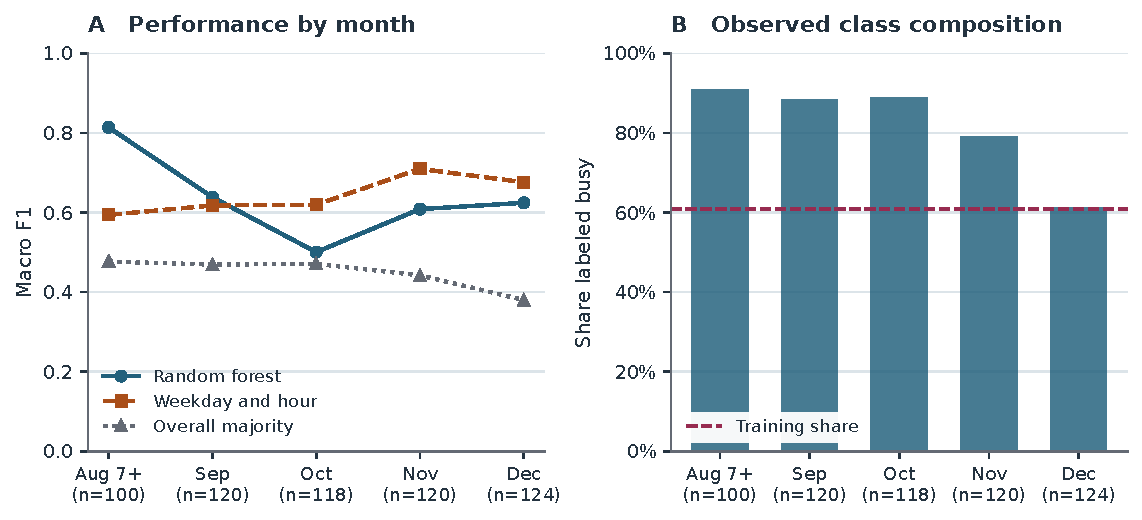
\includegraphics[width=\linewidth]{bike_monthly.pdf}
\caption{保留期間の月別内訳。左はmacro F1、右は正解ラベルの「混雑」の割合。8月は7日以降。いずれも同じ学習済みモデルと固定したルールに対する記述的な集計で、区間推定は含まない。}
\label{fig:bike}
\end{figure}

図\ref{fig:bike}のとおり、モデルは8・9月、曜日・時間帯のルールは10--12月でmacro F1が高かった。例えば8月は0.814と0.594、10月は0.500と0.619である。混雑の割合も8月91.0\%から12月61.3\%まで変化した。この観察から、後続期間全体の集計と、月別のクラス構成と結果を併記する意義が分かる。変化の原因と時系列の依存を考慮した差の区間は、本実験からは確定できない\cite{audit,milestone}。

\section{補足実験}\label{sec:additional}

\subsection{分類の順位付けとAutoGluonとの照合}

IrisとWineでは、5分類器を学習側の共通分割で比較した。共通の分割を変えて繰り返すと、点順位に加え、反復間の順位の変動を確認できる。順位付けと別に保留した比較用データを用いたWineの例では、他の4候補とCV首位との差の95\%区間がいずれも0を含んだ。これは指定した比較用標本での結果である\cite{ranking,worklog}。

AutoGluon Tabular 1.6.3との比較では、同じ外側のCV分割と最終テストを使った。AutoGluonは各外側foldの学習範囲内で内部検証を行い、外側の評価前に学習範囲全体に再適合した。比較した候補はRandom Forest、Extra Trees、k近傍法、ロジスティック回帰、加重アンサンブルである。LightGBMの試行は実行前の空きメモリ確認で見送った。各ワークフローは候補、前処理、実装が異なるため、同じ分類器の一致試験とは範囲が異なる\cite{agcheck}。

\begin{table}[htbp]
\centering
\small
\caption{同じ最終テスト行でのAutoGluonとDIY AutoMLの照合。差はAutoGluonのmacro F1からDIY AutoMLの値を引いたもの。}
\label{tab:autogluon}
\begin{tabularx}{\linewidth}{@{}p{24mm}YYl@{}}
\toprule
題材 & DIY AutoMLの選定モデルとF1 & AutoGluonの選定モデルとF1 & 差の点推定と95\%区間 \\
\midrule
Iris（30行） & SVM / 0.9666 & k近傍法 / 1.0000 & $+0.0334\ [0.0000,\,0.1023]$ \\
Wine（36行） & SVM / 0.9710 & ロジスティック回帰 / 0.9710 & $0.0000\ [-0.0911,\,0.0911]$ \\
\bottomrule
\end{tabularx}
\end{table}

Irisの差の区間は0に達し、Wineでは0をまたいだ。Wineの混同行列が一致しても、誤分類した行は二つの方法で異なった。選定後の予測に条件付けた区間と、小規模な開発用データの範囲で読む必要がある。

\subsection{深層学習バックエンドと予測確率}

WindowsのCPU上でTensorFlow CPU 2.20.0、Keras 3.15.1とPyTorch 2.14.0を比較した。IrisとWineに対し、同じ分割、標準化、MLPの構成（隠れ層32、16、8）、初期重み、ミニバッチ順を用い、学習seed 42、43、44でそれぞれ学習した。共通重みの推論と、両バックエンドで独立に学習した後の予測を分けて照合した\cite{dlcheck}。

共通重みでの最大確率差は概ね \(6\times10^{-8}\) だった。学習後のテスト行・クラス・seed全体での最大絶対確率差は、Irisで0.03053、Wineで0.00211だった。両データの分類ラベルは各seedで行ごとに一致し、macro F1も一致した。予測確率を費用や閾値の計算に使う場合は、ハードラベルで確認できた一致に加え、確率の差と校正を調べる余地がある。

保存済みlogitから計算した3 seed平均のlog loss差（PyTorchからTensorFlowを引く）はIrisで \(-0.002212\)、Wineで \(-0.00006439\) だった。Irisの1,000回の行再標本化による95\%区間は \([-0.005877,\,0.000602]\) だった。Wineでは同じ乱数列を1,000回から20,000回に延ばすと、区間の上端が \(-3.0\times10^{-7}\) から \(+1.8\times10^{-7}\) に変わった。反復数の変更は、同一予測に条件付けた区間の数値的な変動を確認する操作である。独立な学習データや追加のseedによる新しい検証は別途必要になる\cite{dlprob}。

\subsection{数値計算と仮の校正ずれ}

順位付けの検証では、保持した分類器のテスト入力をFloat32へ丸めてから戻し、IrisとWineの予測ラベルに変化がないことを確認した。Irisでテストの花弁幅すべてに \(+0.5\) cmを加える仮定では、30件中6件で予測が変わり、macro F1は0.9666から0.7341へ変わった。前者は指定した丸め、後者は一定の入力オフセットに対する感度である。実際の測定の偏り、推論器の全演算を低精度にした場合、分布の変化は、条件を変えた別の検証で扱う\cite{ranking,worklog}。

\subsection{Annealing checkによる任意の特徴量探索}

Annealing checkは、分類器を固定して特徴量の部分集合を選ぶCPUの任意実行である。焼きなまし法\cite{kirkpatrick}の近傍は1列の追加・削除、または1列の交換で作る。探索に使う指標は共通の学習側CVでのmacro F1である。比較には同じ候補評価数のランダム探索と全列モデルを置き、小さい探索空間では全列挙も照合に使う。候補、温度、受理の経過と実際の学習回数を保存する\cite{annealing}。

Irisでは4特徴量の非空15候補を全列挙し、全列のCV F1 0.9707が最高だった。各手法8候補の予算で、10探索seedのうち焼きなまし法は3回、ランダム探索は8回、このCV最良値に達した。Wineでは13特徴量から最大6列を選び、手法ごとに32候補、320回のCV学習を割り当てた。CVでは各手法が10探索seedのうち5回ずつ上回った。IrisとWineの各seedで、保留macro F1の焼きなまし法とランダム探索の差に付けた95\%区間は0を含んだ。共通の保留標本で探索seedを変えた結果なので、10回を独立な外部検証として数えない。量子アニーリングとQUBOは別の研究課題に残す。

\subsection{16\,GBのWindows端末での点検と学習}

Windows、Intel Core i5-14400、物理メモリ約16\,GB、Python 3.13.17の端末で、模擬数値CSVの点検、作業用Parquetへの変換、選択行の抽出、抽出後のモデル比較を個別に測った。固定seedで整数特徴量を作り、一部の加重和から二値ラベルを作った。各工程を3回実行し、時間はCLI起動から終了までの中央値とした。BLASとOpenMPは1スレッドとし、ピークメモリはCLIプロセスのワーキングセットで測った\cite{scalebench}。

\begin{figure}[htbp]
\centering
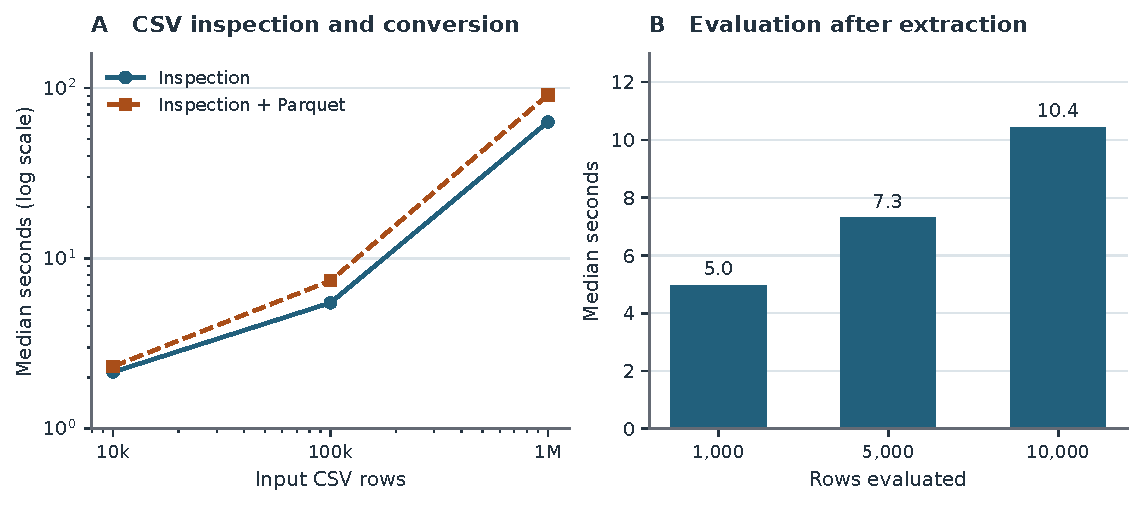
\includegraphics[width=\linewidth]{processing_cost.pdf}
\caption{模擬データの処理時間。左は7特徴量のCSV点検と作業用Parquetへの変換で、両軸を対数表示。右は7特徴量の抽出済みCSVに対する5モデルの比較・保留評価・保存の所要時間。各値は工程ごとに3回測った中央値。}
\label{fig:scale}
\end{figure}

100万行・7特徴量のCSVは36.2\,MB、作業用Parquetは18.9\,MBだった。点検だけは63.3秒、点検と変換は91.1秒を要した。作成済みParquetから2条件を満たす先頭1万行を抽出する工程は2.3秒で、5モデルの比較と保留テストを含む評価工程は10.4秒だった。5,000行では7特徴量の評価が7.3秒、28特徴量が11.6秒だった。100万行は点検・保存の規模であり、学習を計測した最大規模は1万行である。図\ref{fig:scale}はこの端末と数値データの結果で、データ型、列数、ファイルキャッシュ、実行するモデルが変われば負荷も変わる。

\section{考察}\label{sec:discussion}

\subsection{何を分けて評価するか}

Iranian Churnの例では、行単位で分けると同じ入力値を持つ保留行が107件あった。グループ分割は、その数を0にする要件を満たした。同じ入力をまとめても、解約のような異なる結果が同じ組に現れ得るため、重複除去とは挙動が異なる。顧客単位の一般化を問うときに、顧客IDが得られるなら、そのIDに基づく分割を優先して考える。数値入力の一致で作るグループは、抽出した特徴量が変わると変化する。入力の重なり指標も、選んだ列と基準を添えて読む。

自転車貸出の観測では、後の期間でも時刻や稼働日の値は繰り返される。今回確保した境界は日付の境界であり、学習に含まれない暦特徴量の組を作ることとは異なる。時間的な一般化を調べる場合、同じ観測日は分けず、評価期間の開始前に得られた特徴量と正解だけを使えることを確認する必要がある。

\subsection{単純ルール、誤りの内訳、採用判断}

自転車貸出では、曜日・時間帯ルールが全保留期間のmacro F1で上回り、モデルは少数側の「通常」をより多く検出した。誤検知も増えたため、どの誤りを減らしたいかを決めてから数値を比較する必要がある。また、月別のクラス構成も異なり、8月は月初の一部を含まない。月のmacro F1を平均した値は、582行をまとめて混同行列を作った全期間のmacro F1と集計の意味が異なる。比較レポートには両方の分母と対象期間を残す。

評価基盤は、入力データと記録された評価条件から求めた順位、スコア、誤りの内訳を提示する。実務上の採用は利用者が決める。たとえば、交差検証でAのスコアが最も高く、利用者がBを採用する場合は、共通の分割と指標で求めたBとAの差を示せる。保留テストで差を求めるには、両者を同じ保留データに適用した評価が必要になる。

実務への適用では、単純ルールの定義と利用できる特徴量を評価前にそろえ、別期間または別集団で確かめる。自転車のルールは最初の保留結果の確認後に選んだ探索的比較である。したがって、将来の運用を決めるには、同じ比較を事前に固定した追加の後続期間が要る。分類の採用価値を議論するには、見逃しと誤検知の費用、確率の校正、運用時の閾値、実際の施策による結果も必要になる。

\subsection{区間の範囲と再現性}

固定モデルの区間は、観測した行またはグループの再標本化が指標に与える変動を示す。行間やグループ間の依存、データの代表性、特徴量選択やモデル選定までやり直した場合の変動は、評価設計を変えて調べる。日付順の比較では、連続する観測日の依存と観測日の欠落を扱える方法が必要である。連続日をまとめるブロック・ブートストラップ\cite{kuensch}を候補とし、定常性を近似できる期間とブロック長への感度を検討する。十分な観測日を確保し、同じ保留対象に対するモデルとルールの差を集計することが今後の課題である。

保存した入力のハッシュ、分割、予測、設定は、結果の再計算と入力改変の検出に使える。WindowsとPythonでの検証、独立した環境での過去の実行照合、保存したExcelの再計算は、実装の動作と実行再現性に関する証拠である。対象業務の分布への一般化は、時点や組織を変えた追加データから検証する。

\section{結論}

\project{}は、点検したCSVから評価条件を明示し、学習側でモデルを選び、保留テストで単純ルールと誤りの内訳を比較して結果を保存する手順を構築した。通信解約では、特徴量が完全に一致する行をまとめる効果を確認した。自転車貸出では、曜日・時間帯の多数決が全期間のmacro F1で、選定モデルが一部の月と「通常」の検出件数で上回った。日付順に分け、分割、単純ルール、誤りを並べて調べたことで、単一の性能値では見えにくい違いを記録できた。

次は、日付順の分類評価に合わせた性能差の区間と、正解ラベルが遅れて確定する用途の分割を整える。続いて、データ量を変えた学習曲線、学習と選定をやり直した場合の変動、BP画面の初回利用者による結果の読み取りを検証する。

\clearpage
\appendix
\section{再実行の入口}\label{sec:repro}

実装の参照点はGitHubのコミット \texttt{80b25cc} である。分類評価、既存の図付きExcel、入力と分割、設定はこのコミットと付属資料を参照する。マイルストーンでは Windows と Python 3.13.17 で全246テストが通過した。保存した行単位・グループ単位・日付順評価と図付きExcelも照合した\cite{milestone}。この件数はソフトウェアの動作検証であり、独立した業務事例の件数とは別である。

\subsection{入力の準備}

\begin{itemize}
  \item 業務3例の抽出条件、特徴量名、ランダムseedおよび単純ルールは実験記録に固定されている。ホテル・カフェ券の抽出seedは20261108、保留分割seedは42、再標本化seedは43である。カフェ券のルールは、月1回以上のカフェ利用を条件に、急ぎの行き先がなく子どもも同乗していない場合、または有効期限が1日の場合に受取とした\cite{business}。
  \item Iranian Churnの比較は元の3,150行を保ち、節\ref{sec:experiments}に示した7列と正解ラベルを元の行順でCSVへ出す。表\ref{tab:churn}の再現にはこの入力を使う。2,754行の予備試行で用いた削除・集約は別手順である\cite{audit,churnpilot}。
  \item Bike Sharingでは \texttt{hour.csv} の8・12・16・20時を抽出する。\texttt{dteday} と \texttt{hr} からISO形式の観測時刻 \texttt{observed} を作り、\texttt{hr}、\texttt{mnth}、\texttt{workingday} を数値特徴量とする。\texttt{cnt} が200以上ならラベルを \texttt{busy}、それ以外を \texttt{regular} とする。元の結果では入力順に依存しないことを点検するため、Pythonの \texttt{random.Random(42)} で行を並べ替えた\cite{audit}。
\end{itemize}

\subsection{分類評価と保存結果の確認}

仮想環境からリポジトリのルートで実行する例を示す。改行はBashの継続記号で表した。PowerShellでは各コマンドを1行にまとめる。ファイル名と出力先は作業環境に合わせる。

{\small
\begin{verbatim}
python -m diy_automl select --csv churn-seven.csv --target Churn \
  --output runs/paper-churn-row
python -m diy_automl select --csv churn-seven.csv --target Churn \
  --group-identical --output runs/paper-churn-group
python -m diy_automl select --csv bike-calendar.csv --target target \
  --time-column observed --output runs/paper-bike
python scripts/validate_selection_run.py runs/paper-bike
\end{verbatim}
}

Windowsの画面は \texttt{python -m diy\_automl bp-preview} で起動できる。日付順の出力では、\texttt{report.xlsx} の \texttt{SL\_Test\_Comparison}、\texttt{SL\_Test\_By\_Month}、\texttt{SL\_Test\_By\_Month\_Class} を使う。日本語の評価Excelにも対応するシートがある。学習行、保留行、予測は \texttt{arrays.npz}、クラス順と分割の設定は \texttt{manifest.json} で照会する\cite{audit,milestone}。

本稿の図\ref{fig:bike}と図\ref{fig:scale}は、保存済みの評価表と計測JSONから抜き出した集計値を使って作成した。TeXプロジェクトに集計値と描画スクリプトを同梱する。描画の再実行にモデルの再学習は要らない。AutoGluon、DLバックエンド、Annealing checkの再実行条件と設定は各検証記録を参照する\cite{agcheck,dlcheck,annealing,scalebench}。

\newcommand{\record}[2]{\href{https://github.com/okamasaya/DIY_AutoML/blob/80b25cc/#1}{#2}}
\begin{thebibliography}{99}
\small
\raggedright
\setlength{\itemsep}{0.18\baselineskip}
\setlength{\parsep}{0pt}

\bibitem{autogluon}
N.~Erickson, J.~Mueller, A.~Shirkov, H.~Zhang, P.~Larroy, M.~Li, and A.~Smola.
\textit{AutoGluon-Tabular: Robust and Accurate AutoML for Structured Data}.
\href{https://arxiv.org/abs/2003.06505}{arXiv:2003.06505}, 2020.

\bibitem{letters}
DIY AutoML.
\textit{モデル選定と条件付き不確かさ評価を接続する評価基盤}.
\href{https://github.com/okamasaya/DIY_AutoML/blob/c45c0b2/docs/letters/DIY_AutoML_Letter_20261109.pdf}{11月9日試読版}、
\href{https://github.com/okamasaya/DIY_AutoML/blob/c45c0b2/docs/letters/DIY_AutoML_Letter_20261119_review.pdf}{11月19日改稿案}、2026年。

\bibitem{milestone}
DIY AutoML.
\record{docs/BP_CLASSIFICATION_MILESTONE_20261119.md}{BP版の分類評価マイルストーン}、2026年11月19日。

\bibitem{audit}
DIY AutoML.
\record{docs/DATA_AUDIT.md}{学習前の点検、列抽出、分類評価の操作と検証}、コミット \texttt{80b25cc}。

\bibitem{ranking}
DIY AutoML.
\record{docs/SL_UNCERTAINTY_AUDIT.md}{分類結果の不確かさを点検する}、コミット \texttt{80b25cc}。

\bibitem{varma}
S.~Varma and R.~Simon.
Bias in error estimation when using cross-validation for model selection.
\textit{BMC Bioinformatics}, 7:91, 2006.
\href{https://doi.org/10.1186/1471-2105-7-91}{doi:10.1186/1471-2105-7-91}.

\bibitem{groupkfold}
scikit-learn.
\href{https://scikit-learn.org/stable/modules/generated/sklearn.model_selection.StratifiedGroupKFold.html}{StratifiedGroupKFold}.
API documentation.

\bibitem{efron1979}
B.~Efron.
Bootstrap Methods: Another Look at the Jackknife.
\textit{Annals of Statistics}, 7(1):1--26, 1979.
\href{https://doi.org/10.1214/aos/1176344552}{doi:10.1214/aos/1176344552}.

\bibitem{hoteldata}
N.~Antonio, A.~de Almeida, and L.~Nunes.
Hotel booking demand datasets.
\textit{Data in Brief}, 22:41--49, 2019.
\href{https://doi.org/10.1016/j.dib.2018.11.126}{doi:10.1016/j.dib.2018.11.126}.

\bibitem{coupondata}
UCI Machine Learning Repository.
In-Vehicle Coupon Recommendation [Dataset].
\href{https://doi.org/10.24432/C5GS4P}{doi:10.24432/C5GS4P}.

\bibitem{wang}
T.~Wang, C.~Rudin, F.~Doshi-Velez, Y.~Liu, E.~Klampfl, and P.~MacNeille.
A Bayesian Framework for Learning Rule Sets for Interpretable Classification.
\textit{Journal of Machine Learning Research}, 18(70):1--37, 2017.
\href{https://jmlr.org/papers/v18/16-003.html}{論文}.

\bibitem{retaildata}
D.~Chen.
Online Retail [Dataset].
UCI Machine Learning Repository, 2015.
\href{https://doi.org/10.24432/C5BW33}{doi:10.24432/C5BW33}.

\bibitem{business}
DIY AutoML.
\record{docs/BUSINESS_QUICK_RESULTS.md}{業務3例の探索的評価}。
\record{experiments/business_quick_20261108/protocol.json}{入力と実験条件}、2026年11月8日。

\bibitem{metricunc}
DIY AutoML.
\record{docs/VALIDATION_METRIC_UNCERTAINTY.md}{保存済み分類予測の不確かさ評価の検証}、開発版 0.4.0a6。

\bibitem{churndata}
UCI Machine Learning Repository.
Iranian Churn [Dataset], 2020.
\href{https://doi.org/10.24432/C5JW3Z}{doi:10.24432/C5JW3Z}.

\bibitem{churnpilot}
DIY AutoML.
\record{experiments/bp_churn_pilot/README.md}{通信解約データの準備と予備試行}、2026年11月19日。

\bibitem{bikedata}
H.~Fanaee-T.
Bike Sharing [Dataset].
UCI Machine Learning Repository, 2013.
\href{https://doi.org/10.24432/C5W894}{doi:10.24432/C5W894}.

\bibitem{worklog}
DIY AutoML.
\record{docs/THREAD_SUMMARY_20261118.md}{分類順位・分類品質・誤差点検の作業ログ}、2026年11月18日。

\bibitem{agcheck}
DIY AutoML.
\record{experiments/autogluon_sl_crosscheck/README.md}{AutoGluon Tabularとのクロスチェック}、2026年11月18日。

\bibitem{dlcheck}
DIY AutoML.
\record{experiments/dl_backend_crosscheck/README.md}{TensorFlowとPyTorchのCPU比較}、2026年11月18日。

\bibitem{dlprob}
DIY AutoML.
\record{articles/diy-automl-ds-backend-probabilities.md}{TensorFlowとPyTorchの予測確率とlog lossの追加点検}、2026年11月19日。

\bibitem{kirkpatrick}
S.~Kirkpatrick, C.~D.~Gelatt Jr., and M.~P.~Vecchi.
Optimization by Simulated Annealing.
\textit{Science}, 220(4598):671--680, 1983.
\href{https://doi.org/10.1126/science.220.4598.671}{doi:10.1126/science.220.4598.671}.

\bibitem{annealing}
DIY AutoML.
\record{docs/ANNEALING_CHECK.md}{Annealing checkの設計と検証}、2026年11月19日。

\bibitem{scalebench}
DIY AutoML.
\record{experiments/tabular_scale_benchmark/README.md}{Windowsでの表形式データ処理の負荷測定}。
\record{experiments/tabular_scale_benchmark/results-2026-11-19.json}{実測値}、2026年11月19日。

\bibitem{kuensch}
H.~R.~Künsch.
The Jackknife and the Bootstrap for General Stationary Observations.
\textit{Annals of Statistics}, 17(3):1217--1241, 1989.
\href{https://doi.org/10.1214/aos/1176347265}{doi:10.1214/aos/1176347265}.

\end{thebibliography}

\end{document}
